\section{Instances}
	The instances chosen are taken from the exercises done in laboratory, from a Random Generator\footnote{An updated version developed by me of the matrix generation of my colleague Federico Ghirardelli.} of symmetric matrices with board size of 50x50 and by a Random Area Generator.
	
	\paragraph{Random Generator} The Random Generator generate a uniform distribution of points and compute the costs matrix.
	
	\paragraph{Random Area Generator} This generator builds a symmetric matrix that try to represent a real PCB instance. In fact a real PCB instance contains some patterns. I individualized two of this patterns: square frame of points and ordered lines of points. Furthermore there are some random number of points with a random position, it can also be inside an area. 
	
	The generator builds an instance with:
	\begin{itemize}
		\item 3 square frame that have the following characteristics:
			\begin{itemize}
				\item random width and height;
				\item random position in a 50x50 board;
				\item not overlap with others areas;
				\item a random number of points:
				\begin{equation*}
					\frac{P_{tot}}{20} \leq P_{area} \leq \frac{P_{tot}}{5}  
				\end{equation*}
				\item the points inside form a square shape and have equal distance;
			\end{itemize}
		\item 4 lines that have the following characteristics:
			\begin{itemize}
				\item $Height = P_{tot} / 20$;
				\item random position in a 50x50 board;
				\item a random number of points: $3 \leq P_{line} \leq 8$;
				\item constant distance between points.
			\end{itemize}
	\end{itemize}

	The figures~\ref{fig:fakeBoards} show the \verb|fb60| instance and the \verb|fb100| instance used.
	
\newpage
	\paragraph{Instances files}
	The pattern use for naming the file is:
	\begin{center}
		\verb|<group><N>.dat|
	\end{center}
	Where \verb|N| is the number of nodes and \verb|group| meaning the origin of that instances.
	
	The instances chosen are (\verb|.dat| is omitted):
	\begin{itemize}
		\item \verb|tsp12|
		\item \verb|tsp60|
		\item \verb|rnd60|
		\item \verb|fb60|
		\item \verb|rnd80|
		\item \verb|fb80|
		\item \verb|rnd100|
		\item \verb|rnd100_2|: build with random generator but with board size 60x60;
		\item \verb|fb100|
	\end{itemize}
	I prefer to select instance with an equal number of nodes but made from different source in order to see how much the instance form impact on the results of meta heuristic methods.
	
	After done this step I took real instances from PCB projects that I will explain in next section \ref{sec:realDomainTests}. 

	\begin{figure}[hb]
		\centering
		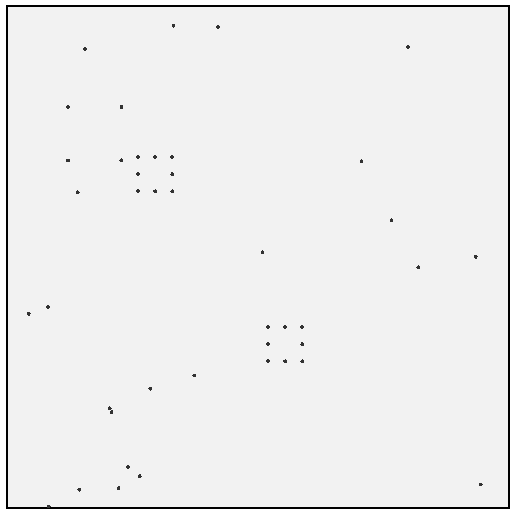
\includegraphics[width=0.44\textwidth]{img/fb60}%
		\qquad\qquad
		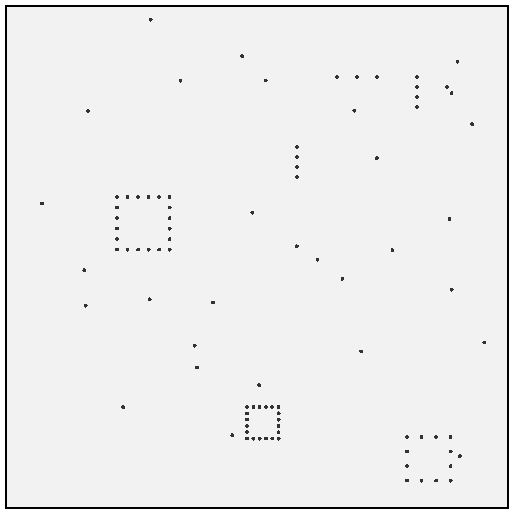
\includegraphics[width=0.44\textwidth]{img/fb100}
		\caption{Random fake PCB with 60 and 100 nodes}
		\label{fig:fakeBoards}
	\end{figure}